\documentclass[12pt,a4paper]{report}

% English
\usepackage[english]{babel} % English language setting
\usepackage[utf8]{inputenc} % Unicode text
\usepackage[T1]{fontenc} % German 'Umlaute'
\usepackage{textcomp} % Euro
\usepackage[hyphens]{url}
\usepackage{amssymb} % Symbols
\usepackage{emptypage} % Empty pages are now actually empty

% Fonts, with all the options
\usepackage{mathpazo}
\usepackage[scaled=.95]{helvet}
\usepackage{courier}
\usepackage{microtype}

% Images and listings
\usepackage{graphicx} % images
\usepackage{subfig} % sub-figures
\usepackage{wrapfig} % wrapping figures
\usepackage{listings} % better source code listings
\usepackage{enumitem}
\graphicspath{ {figures/} }

% Source code
\usepackage{float}
\newfloat{listing}{htbp}{scl}[chapter]
\floatname{listing}{Listing}
\usepackage{packages/coding/golang/lang} % import this package after listings
\usepackage{packages/coding/protobuf/lang}  % include language definition for protobuf
\usepackage{packages/coding/protobuf/style} % include custom style for protobuf declarations.
\lstset{
    basicstyle=\scriptsize\ttfamily,
    columns=[l]flexible,
    mathescape=true,
    showstringspaces=false,
    numbers=left,
    numberstyle=\tiny,
    frame=none,
    keywordstyle=\color{red},
    stringstyle=\color{blue},
    showstringspaces=false,
    tabsize=4,
    xleftmargin=\leftmargin,
    language=Golang
}

% Page layout
\usepackage[paper=a4paper,width=14cm,left=35mm,height=22cm]{geometry}
\usepackage{setspace}
\usepackage[htt]{hyphenat}
\usepackage{sectsty}
\linespread{1.5}
\subsubsectionfont{\large}

% Page markers
\newcommand{\phv}{\fontfamily{phv}\fontseries{m}\fontsize{10}{12}\selectfont}
\usepackage{fancyhdr} % nicer header and footer
\pagestyle{fancy}
\renewcommand{\chaptermark}[1]{\markboth{#1}{}}
\fancyhead[L]{\phv \nouppercase{\leftmark}}
\fancyhead[R]{\phv \thepage}
% rather not use anything for the footer
\fancyfoot[C]{\ } % no page count in the bottom
%\fancyfoot[R]{\textsf{\small Media Management}}

% Share the sources
\usepackage{bibtopic}

% Logo of the university
\usepackage{packages/hsrmlogo}

% Special packages
\usepackage{epigraph}
\setlength{\epigraphrule}{0pt} % no divider
\usepackage{csquotes}

% Some extra styles
\usepackage{soul}
\newcommand*\strikethrough{\st}

% Hyperlink everything
\usepackage{hyperref}
\hypersetup{
    bookmarks=true,
    colorlinks=true,
    linkcolor=black,
    citecolor=black,
    filecolor=black,
    urlcolor=black,
}
\urlstyle{same}

% Wikipedia-style "citation needed" macro
\newcommand{\cn}[1][]{\textsuperscript{\color{red} ~[citation needed]~}}

% Code markup
\newcommand{\code}[1]{\texttt{#1}}


\newcommand{\studyprogramme}{Media Management}
\newcommand{\degreetype}{Bachelor of Arts}
\newcommand{\thesistitle}{
The system and software architecture of back-end applications for the short-term rental of electric scooters
}
\newcommand{\thesissubtitle}{
Analysis of an existing solution and evaluation on the potential of its augmentation
}
\newcommand{\thesisauthor}{Jakob Löhnertz}
\newcommand{\thesisdate}{23. Juli 2018}
\newcommand{\thesislocation}{Wiesbaden}
\newcommand{\firstmarker}{Prof.\ Dr.\ Johannes Luderschmidt}
\newcommand{\secondmarker}{Merle Hiort}

\begin{document}

\begin{titlepage}
  \begin{center}
    \hsrmlogo[1]
    \parbox[t]{8cm}{
      Hochschule \textbf{RheinMain}\\
      Fachbereich Design Informatik Medien\\
      Studiengang \studyprogramme}
    \\[1.5cm]
    {\LARGE Abschlussarbeit} \\[0.5cm]
    {\begin{spacing}{1} \large zur Erlangung des akademischen Grades \\[5mm] \end{spacing}}
    {\begin{spacing}{1} \large \degreetype \\[1cm] \end{spacing}}
    \rule{\textwidth}{1pt} \\[0.5cm]
    {\begin{spacing}{1.15} \huge \bfseries \thesistitle \\ \end{spacing}}
    {\begin{spacing}{1.15} \bfseries \thesissubtitle \\[0.60cm] \end{spacing}}
    \rule{\textwidth}{1pt}
    \\[1.5cm]
    \begin{tabular}{ll}
      Vorgelegt von & \thesisauthor \\
      am & \thesisdate \\
      Referent & \firstmarker \\
      Korreferent & \secondmarker
    \end{tabular}
  \end{center}
\end{titlepage}
\cleardoublepage

% Erklärung gemäß den Allgemeinen Bestimmungen für Prüfungsordnungen
\thispagestyle{empty}
\section*{Erklärung gemäß ABPO}
Ich erkläre hiermit, dass ich
\begin{itemize}
\item die vorliegende Abschlussarbeit selbstständig angefertigt,
\item keine anderen als die angegebenen Quellen benutzt,
\item die wörtlich oder dem Inhalt nach aus fremden Arbeiten entnommenen
  Stellen, bildlichen Darstellungen und dergleichen als solche genau
  kenntlich gemacht und
\item keine unerlaubte fremde Hilfe in Anspruch genommen habe.
\end{itemize}

\vspace{6em}
\noindent\begin{tabular}{p{0.37\textwidth}p{0.56\textwidth}}
\thesislocation, \thesisdate  & \rule{0.56\textwidth}{0.5pt}\\
              & \makebox[1cm]{\ } \thesisauthor
\end{tabular}

\vfill

\cleardoublepage



\begin{abstract}

The abstract will be added at this place towards the end of the thesis.

\end{abstract}


\tableofcontents



\chapter{Problems and research question} \label{chap:intro}

\epigraphhead[55]{\epigraph{Beauty is more important in computing than anywhere else
in technology because software is so complicated. Beauty is the ultimate defense against complexity.}
{\textit{David Gelernter}}}


The definition of the word \emph{scooter} is fairly vague.
Some describe it as a small vehicle with a handlebar and a platform to stand on,
the kind traditionally children were riding.
However, this paper looks at the \emph{motorcycle-esque type} of a scooter, and in
particular the electric version of it.\\
Many pain points of internal combustion engines vanish with the switch to their electric
counterparts. The maintenance of the mechanical system of the whole vehicle becomes easier.
There are less moving parts which makes for less errors.
On the downside, the exchange of the fuel causes the most problems with electric engines.
Of course they utilize batteries instead of fossil fuels as their impetus.
Although the invention of the battery is older than that of the
internal combustion engine\cn, the technology is still not perfected and sees new
advancements every year. Alas, it also combats many challenges in terms of
safety, cost, capacity, weight, recycling, speed of recharging and longevity.\\
For the provider, the handling of a short-term rental service
only becomes feasible with the automation of as many processes as possible.
This requires a back-end application ideally paired with a front-end.
Most of the time, ongoing human resource costs make up the biggest percentage
in the expenses of any business.\cn Thus, this demands for less human workforce
as part of the processes of a rental service.
Meanwhile, the upfront expenditures for the software development of
an application are still vast but in the long run, the running expenses are less.
The only cost driver afterwards is the maintenance of the created software.
As a consequence, the question should be how to mitigate the maintenance costs
of a software product. The main aspect is a proper application of
software engineering which is defined as:
\begin{displayquote}
\emph{"The application of a systematic, disciplined, quantifiable approach to the
development, operation, and maintenance of software."}~\cite{se-ieee}
\end{displayquote}
To put this definition into words, software engineering mainly targets
the domains of software architecture, code quality and documentation.\cn\\
All of these pursue one long-term goal: to achieve a well functioning, maintainable
software product.
Furthermore, the fact that the scooters are always connected to the internet
as well as the nature of current batteries desire a reactive and faultless application.\\
Finally, the corporate partner of this thesis, which is discussed in detail
in section \ref{sect:kumpan}, is already in possession of a solution which is not fully featured yet.
Therefore, the subject of augmenting an existing back-end application with missing features is also targeted.\\
To conclude, this leads into the research question of this bachelor thesis:\\
\emph{Which functional modules are necessary for the implementation of a back-end application
for the short-term rental of electric scooters and which considerations need to be made
to integrate additional functionality into an existing legacy software solution for that purpose?}



\chapter{Fundamentals} \label{chap:fundamentals}

\epigraphhead[55]{\epigraph{The danger in the sequence [waterfall approach]
is that the project moves from being grand to being grandiose,
and exceeds our human intellectual capabilities for management and control.}
{\textit{Harlan D. Mills}}}


\section{The market for the rental of electric scooters}

The market for the short-term rental of motor vehicles in Germany
is currently growing rapidly~\cite{bundesverband-carsharing-statistics}.
The situation on the market is no different for medium and long-term rentals.~\cite{sparkasse-kfz-vermietung}
However, this sector is dominated by cutthroat competition.
It has been dictated by large corporations such as \textit{Sixt}, \textit{Hertz},
\textit{Avis} and \textit{Europcar} for years.~\cite{sparkasse-kfz-vermietung}
Although smaller providers exist, this market has become an oligopoly and
the barriers for a market entry are high for new types of providers.
In contrast, the market for short-term rental, also known as car sharing for cars,
is a comparatively young market. It has only existed in Europe in its breadth
since the late 1980s~\cite{history-of-carsharing} and in its current form
only since the advent of the smartphone, since many offers require the use of a mobile app.
For this reason the market for short-term rentals and thus its saturation is significantly lower.
According to the \textit{Bundesverband CarSharing e.V.}, the current total number of cars
in the car sharing sector in Germany is about 17,200. In contrast, almost 10\% of all
new vehicle registrations in Germany in 2015 were attributable to traditional
car rental companies such as the above.~\cite{sparkasse-kfz-vermietung}
This represents an increase of 339,000 vehicles, in similar fashion every year.
By contrast, the share of vehicles with electric drive is again lower at
just under 10\% of the total number of car sharing vehicles.
Electric scooters do not even appear in the statistics of the
\textit{Bundesverband CarSharing e.V.}~\cite{bundesverband-carsharing-statistics}\\
However, the market in other nations has already experienced strong growth;
one example is the Chinese market. Around 20 million electric scooters were sold
there in 2016 alone.~\cite{heise-electric-scooters}
Additionally, the short-term rental of these is already a working business model
in China.~\cite{allchinatech-electric-scooters} Market value forecasts are also promising.
Last year, the US company \textit{P\&S Market Research} predicted an annual growth of
just under 7\% in the market for motorized two-wheeled vehicles with
electric drive until 2025.~\cite{pands-electric-scooters}
The totality of these figures and the status quo in China create a positive impression
with regard to the possibility of a successful market entry into this sector in Germany.
The future of the market is also promising, as more and more nations around the world
are deciding on a ban on vehicles with internal combustion engines for the
foreseeable future~\cite{faz-combustion-engine-ban} and companies already
in the market are undertaking their first expansions.~\cite{allchinatech-electric-scooters, faz-electric-scooters}


\subsection{German electric scooter manufacturer \textit{Kumpan}} \label{sect:kumpan}

The thesis loosely focuses on the business of German electric scooter manufacturer \textit{Kumpan}.
The company was established in 2009. For their product, they concentrated on three main aspects:
an exterior design ready for the European market, build quality and sufficient cruising radius.
They finished building their first electric scooter in 2010 and are thriving for good products ever since.
The price of their electric scooters is still rather high. Owing to that circumstance,
they came up with smaller, cheaper models as well as a completely different approach.\\
Instead of traditional retail sales they started developing the idea of a
short-term rental service for their scooters. And from many angles it makes sense:
As seen in the last section, the market for the short-term rental of electric scooters
especially in Germany is still minuscule compared to e.g. car or bike sharing.
Meanwhile, the costs for buying an electric scooter are still relatively high.
Additionally, many people will not need such a vehicle for the whole day and would benefit
from more flexibility. Lastly, parking spots are also a scarcity in inner cities.
Therefore, \textit{Kumpan} plans to enter the market of short-term electric scooter rentals
in the near future.\\
There are still many aspects to be discussed and determined but one of them
is already set and can be seen as a necessity regardless of the final implementation:
A server back-end application as well as its infrastructure.
\textit{Kumpan} purchased an existing software solution to achieve this.
Beforehand, it was already known though that the software is not feature-complete
for their usage. Thence, it is already planned to augment the software with the missing
features.


\section{Components of a modern software product}

The main aspect of success for such a system is indeed the \emph{magic} behind the scenes
that no customer sees. People just see the electric scooter as the product and
want to be able to ride one on demand by just pushing a button.
The ease of use for the customers and their satisfaction are the main facets
to be considered by the provider of such a service.\\
This, as nearly every modern software product geared towards a general audience,
involves two foundational components --- a front-end and a back-end.~\cite{fischer-lexikon}
On the one hand, the front-end provides the user interface of the product, the façade of the whole.
It is the component the customer interacts with but more importantly it will be
what the users identify the product with.
On the other hand, the back-end is the brain of the software product.
It provides endpoints for the front-end to use and consume. The back-end dictates
what the front-end will do. Meanwhile, it does not determine what it will look like.
If the front-end is unusable the back-end will never be able to fix that as the
front-end becomes the mental representation of the whole product for the customers.
If the back-end behaves sluggish or is prone to errors, the front-end will not be able to save much
by the same token. In the end, both form a synergy with each other.\\
This thesis will shed light on the back-end of such an application.
It will focus on the software architecture of it.
This includes the functionalities that are mandatory and the question on how the product
might come together; from ideas and drafts to written source code.


\subsection{Necessity of a thorough back-end application}

A look at existing car sharing offers depicts that automating the rental process
is necessary. There are three main aspects that become easier to achieve for the
provider if they choose to automate their system.\\
Firstly, as already mentioned in the first chapter,
the costs are a lot lower whenever less human resources are involved.
Additionally, the speed of execution of a rental request by a customer gets better
with a performant back-end application.
Finally, a modern software solution attracts more customers as the ease of use
is expected to be better. Furthermore, the entrance barrier to try a rental service
gets lower. Nowadays, customers, especially younger ones, are used to web-based
or mobile app-based software and are a lot more likely to try out such an offer.~\cn
Although, the users are never in contact with the back-end, it is absolutely
crucial for the success of the whole application as the front-end just displays
the information in a presentable way while not performing any serious
business logic most of the time.


\section{Approaching the development of software}

From a very fundamental standpoint, software development consists of two distinct phases.
The planning and analysis phase which leads into the programming phase.~\cite{royce-large-systems}
Upon further investigation, there are more steps before, in between and after these two essential ones.
In his influential 1970 paper \textit{"Managing the Development of Large Software Systems"},
American computer scientist Winston W. Royce discusses his idea of a satisfactory
software development process. His paper is often mistakenly cited as the starting point
of the \textit{waterfall model} whereas Royce indeed starts his paper with such an approach but quickly
depicts the shortcomings of that model.~\cite{royce-large-systems, larman-iid-history}
The waterfall model describes the idea that a software development process should consist of
the stages shown in figure \ref{fig:waterfall-model}.
\begin{figure}[htb]
\centering
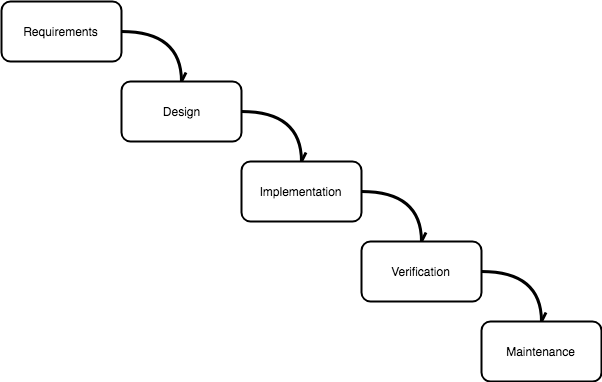
\includegraphics[width=.60\textwidth]{waterfall-model}
\caption{The essential stages of the waterfall model}
\label{fig:waterfall-model}
\end{figure}
The main point of it is that the steps are conducted sequentially; no step should
begin before the current one has been finished.~\cite{boehm-spiral}
This idea has one big flaw: the \textit{Verification} phase being nearly at the end.
Only after the whole software product is finished, an evaluation by internal testing personnel or
the client can be carried out.~\cite{royce-large-systems}
It is likely that at least some changes to the implementation will be necessary after the \textit{Verification}.
Additionally, clients may not know the exact requirements at the very beginning
of the software development process.~\cite{parnas-rational-design-process}
It is also possible that a major fault is only discovered in that second last stage ---
the negative repercussions could be massive.
\begin{displayquote}
\emph{"Either the requirements must be modified, or a substantial change
in the design is required. In effect the development process has returned to
the origin and one can expect up to a 100-percent overrun
in schedule and/or costs."}~\cite{royce-large-systems}
\end{displayquote}
Nevertheless, the idea Royce describes is what made his paper as influential.
The steps that are required to get from an idea to a finished product nearly always
stay the same. The ones from figure \ref{fig:waterfall-model} are still applicable to
many newer concepts of a software development process.
Nowadays, software developers and project managers are mostly utilizing any model that
can be subsumed under the loose term \textit{agile}.
In summary, as the term already depicts, this theory is geared towards
the idea that the software development process should not be as rigid and constrained.
Therefore, it stands in stark contrast to the demonstrated waterfall model.
The term does not describe a distinct concept but rather an idea ---
there are dozens of implementations of agile software development.~\cite{martin-agile-practices}
Regardless of the implementation, most often agile approaches are based around
the idea of \textit{Iterative and Incremental Development (IID)}.~\cite{larman-iid-history}
\begin{displayquote}
\emph{"Software development should be done incrementally, in stages with
continuous user participation and replanning and
with design-to-cost programming within each stage."}~\cite{mills-iid}
\end{displayquote}
\newpage
Instead of implementing the whole software within all the sequential steps
of the waterfall model, the product is being developed in increments.
Following some initial analyzing and planning, the first iteration begins.
After the end of one iteration of all the steps shown, apart from the \textit{Maintenance},
the next increment is getting projected and eventually executed as shown in figure \ref{fig:idd-model}.
\begin{figure}[htb]
\centering
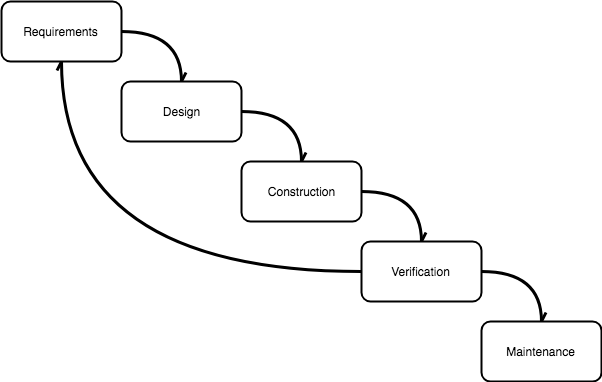
\includegraphics[width=.60\textwidth]{iterative-and-incremental-model}
\caption{A revised, iterative version of the waterfall model e.g. IID}
\label{fig:idd-model}
\end{figure}\\
To conclude, the stages Royce exhibited in 1970 are still applicable today.
In some form or another, those are mandatory for implementing any software.


\subsection{Requirements}

\subsection{Design}

\subsection{Implementation}

\subsection{Verification}

\subsection{Maintenance}



\newpage

% In case the source lists are needed:
\listoffigures
% \listoftables
\newpage

% Separate the sources with 'bibtopic'
\bibliographystyle{plain}
\begin{btSect}{offline}
\section*{References}
\btPrintCited
\end{btSect}
\begin{btSect}{online}
\section*{Online Sources}
\btPrintCited
\end{btSect}

\end{document}
